\documentclass[10pt,a4paper]{article}
\usepackage[margin=23mm]{geometry}
\usepackage{amsmath,booktabs,graphicx}
\usepackage[hidelinks]{hyperref}
\title{Provisional investment before certification}
\author{PARK--REVIVE: controlled financial simulation}
\date{18 October 2026}
\begin{document}\maketitle
\noindent\textbf{Complete sample.} 100 new independent financial markets, seeds
70001--70100, with 500 assets, 100 candidate signals, one initial training year
and 14 out-of-sample years of 252 dates. Every market is retained.
The training rule selects one candidate initially; its fitted target is then
updated annually from past observed returns. This is a controlled first-candidate
timing experiment, not the full adaptive feature-selection fund.

\paragraph{Rules fixed before the new results.}
Provisional exposure is 25\% of the common target when its penalized training
forecast is positive. Training uncertainty uses a Bartlett HAC standard error
with at most 20 lags and a 1.64485 multiplier. This is a working penalty,
without a finite-sample or post-selection confidence guarantee. A 252-day
holding forecast amortizes entry costs; actual performance charges costs when
incurred. The four methods share the candidate and fitting calendar.
Wait holds cash until the shared evidence-and-economic gate; Hybrid invests
provisionally and subsequently uses the common full target. Economic 25\%
and Economic full do not require evidence. Each fund pays its own proportional
and quadratic impact costs; insolvency is absorbing.

\paragraph{Statistical scope.}
The shared nine-component corrected-tail e-process compares the common full
shadow policy with cash at individual level .05. Crossing 20, a positive
historical score mean and favorable current training forecasts are required
at an annual review; execution begins the following trading date.
The certificate does not establish that increasing an existing provisional
position is beneficial. The experiment follows prior pilot observations and
the user discussion; its numerical protocol was committed before these new
market outputs. It is not a pre-pilot registration.

\begin{center}\small
\begin{tabular}{lrrrr}\toprule
Method & Utility & MC SE & Mean wealth & Mean max DD\\\midrule
Wait for evidence & 0.003655 & 0.000581 & 1.057 & 0.25\% \\
Economic 25\% & 0.010747 & 0.000412 & 1.165 & 0.47\% \\
Hybrid 25\% then full & 0.013482 & 0.000805 & 1.217 & 0.63\% \\
Economic full & 0.042602 & 0.001652 & 1.875 & 1.88\% \\
\bottomrule\end{tabular}\end{center}
\noindent Utility denotes mean daily quadratic utility net of actual costs,
multiplied by 252. It is not annual return or certainty equivalent. Wealth
and drawdown are separate compounded outcomes. The primary comparison is
Hybrid minus Wait; the approximate pointwise Monte Carlo intervals below use
the 100 paired markets and Student $t_{99}$, with no simultaneous-coverage claim.
\begin{center}\small
\begin{tabular}{lrr}\toprule
Contrast & Mean & Pointwise 95\% interval\\\midrule
Hybrid minus Wait & 0.009828 & [0.009219, 0.010436] \\
Hybrid minus Economic 25\% & 0.002735 & [0.001872, 0.003598] \\
Hybrid minus Economic full & -0.029119 & [-0.030956, -0.027283] \\
\bottomrule\end{tabular}\end{center}
\noindent Secondary contrasts are unadjusted and descriptive.

\clearpage
\begin{center}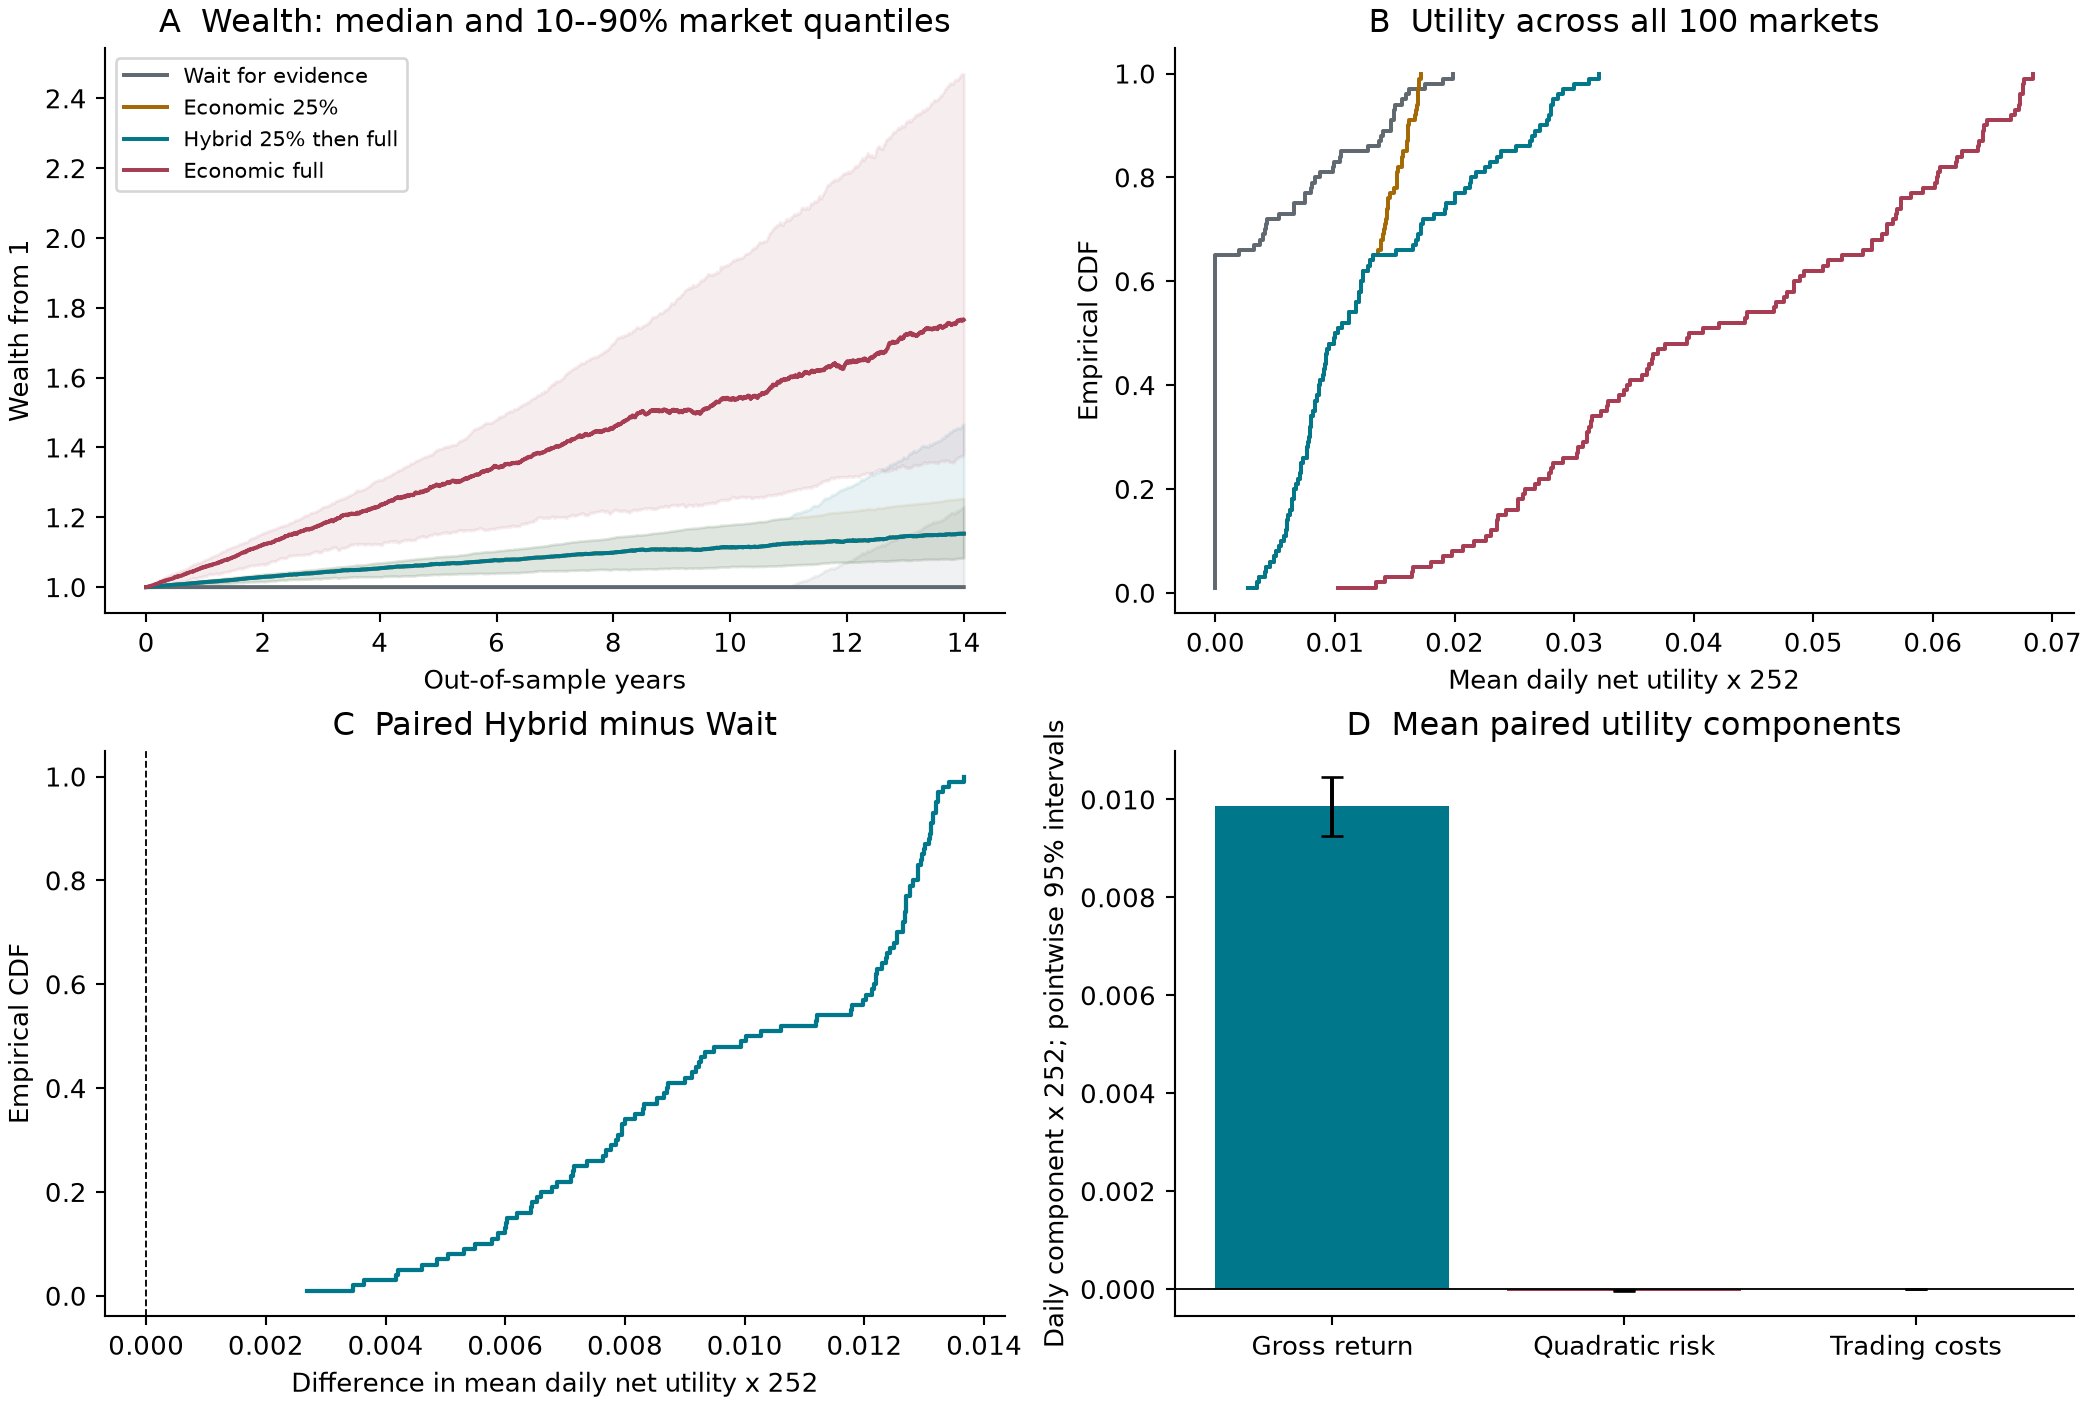
\includegraphics[width=\textwidth]{economic_authorization.png}\end{center}
\noindent All panels use all 100 declared markets. Shading in A shows market
quantiles, not confidence intervals. Panel D decomposes the primary realized
utility gap into gross return, quadratic risk and actual trading costs; its
components sum to that gap. Insolvency, if present, is retained using each
fund's actual executed allocation, so common target paths need not imply
equal positions after a fund fails.

\paragraph{Authorization and downside.}
Initial provisional entry occurred in 100 of 100 markets. The shadow evidence crossed at an annual review in 38 markets; 3 first crossed only at the terminal review. 35 markets executed the common full-exposure authorization. This crossing concerns the shadow candidate versus cash, not statistical certification of the increase from a provisional position. In 0 markets, Hybrid accumulated negative realized utility before the common deployment date (or the full horizon when no deployment occurred). The evaluator counted 784 pre-deployment dates with negative conditional utility for Hybrid. These are descriptive downside measures, not type-I error guarantees or a causal claim about all adaptive selection policies. All 1400 of the 1400 annual target fits were at the leverage cap, and 0 markets changed their target over time. Thus the fitted uncertainty penalty did not produce interior target sizes in this pool. These results evaluate exposure timing for the selected positions; they do not validate the uncertainty calibration or establish the benefit of adaptive position sizing.

\paragraph{Independent verification.}
Policy actions, annual information timing, each fund's costs and wealth,
shadow scores, all nine evidence components and summary metrics were
independently replayed for every market. Two fixed seed identifiers
(70001 and 70002) additionally received complete independent DGP and public
moment-certificate replays. Arithmetic consistency does not establish a
general performance or global multiple-testing guarantee.

\paragraph{Interpretation.}
The paired comparison isolates provisional exposure for the specified
common candidate path, evidence clock and economic gate. Its sign and size
apply to this DGP and rule. Extending conclusions to repeated feature
selection, different uncertainty calibration or other provisional limits
requires a separate evaluation. The ongoing original 500-market fund
study is a different experiment and its markets are not pooled here.
\end{document}
